% Kaelix — verificação de hardware: esquemático, placa, invólucro e simulação
% Compilar:  latexmk -pdf verificacao-hardware.tex
%
% Formato tabular deliberado. Cada linha é um item verificável: o que foi
% medido, com que ferramenta, e o que o resultado permite afirmar.

\documentclass[10pt,a4paper,landscape]{article}

\usepackage[T1]{fontenc}
\usepackage[utf8]{inputenc}
\usepackage[brazil]{babel}
\usepackage{lmodern}
\usepackage[landscape,top=1.5cm,bottom=1.6cm,left=1.4cm,right=1.4cm]{geometry}
\usepackage{booktabs}
\usepackage{tabularx}
\usepackage{array}
\usepackage{siunitx}
\usepackage{amsmath}
\usepackage{microtype}
\usepackage[hidelinks]{hyperref}
\usepackage{caption}
\usepackage{enumitem}
\usepackage{titlesec}
\usepackage{float}
\usepackage{graphicx}
\usepackage{seqsplit}

\sisetup{output-decimal-marker={,}, group-separator={.}, per-mode=symbol}
\captionsetup{font=footnotesize, labelfont=bf}
\setlist{itemsep=1pt, topsep=3pt, parsep=0pt, leftmargin=*}
\titleformat{\section}{\normalfont\large\bfseries}{\thesection}{0.7em}{}
\titlespacing{\section}{0pt}{11pt}{5pt}
\titleformat{\subsection}{\normalfont\normalsize\bfseries}{\thesubsection}{0.6em}{}
\titlespacing{\subsection}{0pt}{8pt}{3pt}
\pagestyle{plain}

% emergencystretch, e não \sloppy: \sloppy dentro do preâmbulo da coluna
% interfere na passada de medição do tabularx e as tabelas encolhem para um
% quarto da largura. O objetivo é o mesmo — impedir que um \texttt de
% caminho de arquivo transborde a coluna.
\newcolumntype{Y}[1]{>{\raggedright\arraybackslash
  \setlength{\emergencystretch}{2em}\hsize=#1\hsize}X}
% \seqsplit ficou de fora: com os pesos de coluna corretos não há
% mais transbordo, e ele espaçava os nomes de arquivo ao justificar.
\newcommand{\arq}[1]{\texttt{#1}}
\newcommand{\ok}{\textsf{fecha}}
\newcommand{\nok}{\textsf{não fecha}}

\begin{document}

\begin{center}
{\Large\bfseries Verificação de hardware do Kaelix}\\[2pt]
{\large Esquemático, placa, invólucro e simulação numérica}
\end{center}

\vspace{2pt}

\section{Escopo e critério}

\begin{itemize}
\item Cobre a cadeia esquemático $\rightarrow$ placa $\rightarrow$ sólido 3D $\rightarrow$ análise numérica, para duas versões (v1, v2) de placa e de invólucro.
\item Nenhum resultado provém de bancada. Todos os valores são de geração, verificação geométrica ou simulação. O documento não reivindica validação experimental.
\item A coluna \textbf{Medição} registra a grandeza que sustenta cada afirmação. Itens sem medição associada aparecem como \textsf{não verificado}.
\item Correções a análises anteriores do projeto constam da Seção~\ref{sec:correcoes} com o valor antigo, o valor corrigido e a causa.
\end{itemize}

\section{Cadeia de geração e verificação}

Nenhum arquivo derivado é editado à mão. A fonte é \texttt{hardware/gen\_schematic.py}.

\begin{table}[H]\footnotesize
\begin{tabularx}{\textwidth}{@{}Y{0.7} Y{1.0} Y{1.3} Y{1.0}@{}}
\toprule
\textbf{Etapa} & \textbf{Ferramenta} & \textbf{Saída} & \textbf{Verificação automática} \\
\midrule
Esquemático & \texttt{gen\_schematic.py} & \texttt{.kicad\_sch}, \texttt{.kicad\_sym}, netclasses & ERC com aviso tratado como erro \\
Placa & \texttt{gen\_pcb.py} + \texttt{router.py} & \texttt{.kicad\_pcb} & DRC com zonas preenchidas; contenção no contorno; colisão mecânica e de cobre \\
Sólido & \texttt{kicad-cli export step}, \texttt{gen\_involucro.py} & \texttt{.step} da placa e do invólucro & existência de modelo por footprint; interferência entre corpos \\
Modal & gmsh 4.15 + CalculiX 2.23 & frequências e formas & convergência de malha em três refinos \\
Térmica & gmsh + CalculiX & campo e transiente & balanço fechado contra modelo concentrado \\
\bottomrule
\end{tabularx}
\end{table}

Regeração a partir de diretório limpo reproduz \texttt{.kicad\_sch}, \texttt{.kicad\_pcb} e \texttt{.kicad\_sym} byte a byte nas duas versões. O roteador é determinístico.

\section{Correções no esquemático}

\begin{table}[H]\footnotesize
\begin{tabularx}{\textwidth}{@{}p{0.7cm} Y{1.184} Y{0.868} Y{0.947}@{}}
\toprule
\textbf{\#} & \textbf{Condição anterior} & \textbf{Medição} & \textbf{Alteração} \\
\midrule
1 & Corte de alimentação dos periféricos por transistor \emph{low-side}. Os pull-ups de \SI{4.7}{\kilo\ohm} permaneciam em +3V3 e alimentavam o MPU6050 pelos diodos de ESD de SDA/SCL & modo de falha FM-27 já registrado em \arq{ANALISE-DE-FALHAS.md} & \emph{Load switch} \emph{high-side} (Q1 SI2301 + Q2 BC847B); pull-ups transferidos para o rail comutado +3V3\_SW \\
2 & MPU6050 permanentemente alimentado & \SI{3.9}{\milli\ampere} contínuos, folha de dados InvenSense & rail comutado; consumo médio do ciclo \SI{314}{\micro\ampere} \\
3 & Ausência de medição de tensão da bateria & REQ-SEG-29 e REQ-SEG-53 dependem dela & divisor \SI{1}{\mega\ohm}/\SI{1}{\mega\ohm} e capacitor de \SI{100}{\nano\farad} em IO6 \\
4 & Ausência de proteção contra polaridade invertida & --- & Q3 SI2301 em série com a entrada \\
5 & Ausência de capacitor no nó do ADC do NTC, embora FM-08 raciocine sobre ``capacitância de filtro $\times$ \SI{10}{\kilo\ohm}'' & \arq{ANALISE-DE-FALHAS.md} & C12, \SI{100}{\nano\farad} \\
\bottomrule
\end{tabularx}
\end{table}

O esquemático é idêntico nas duas versões de placa: mesmos 32 componentes, 24 nets e 118 pads com net. A versão altera contorno, \emph{placement} e roteamento.

\begin{figure}[H]\centering
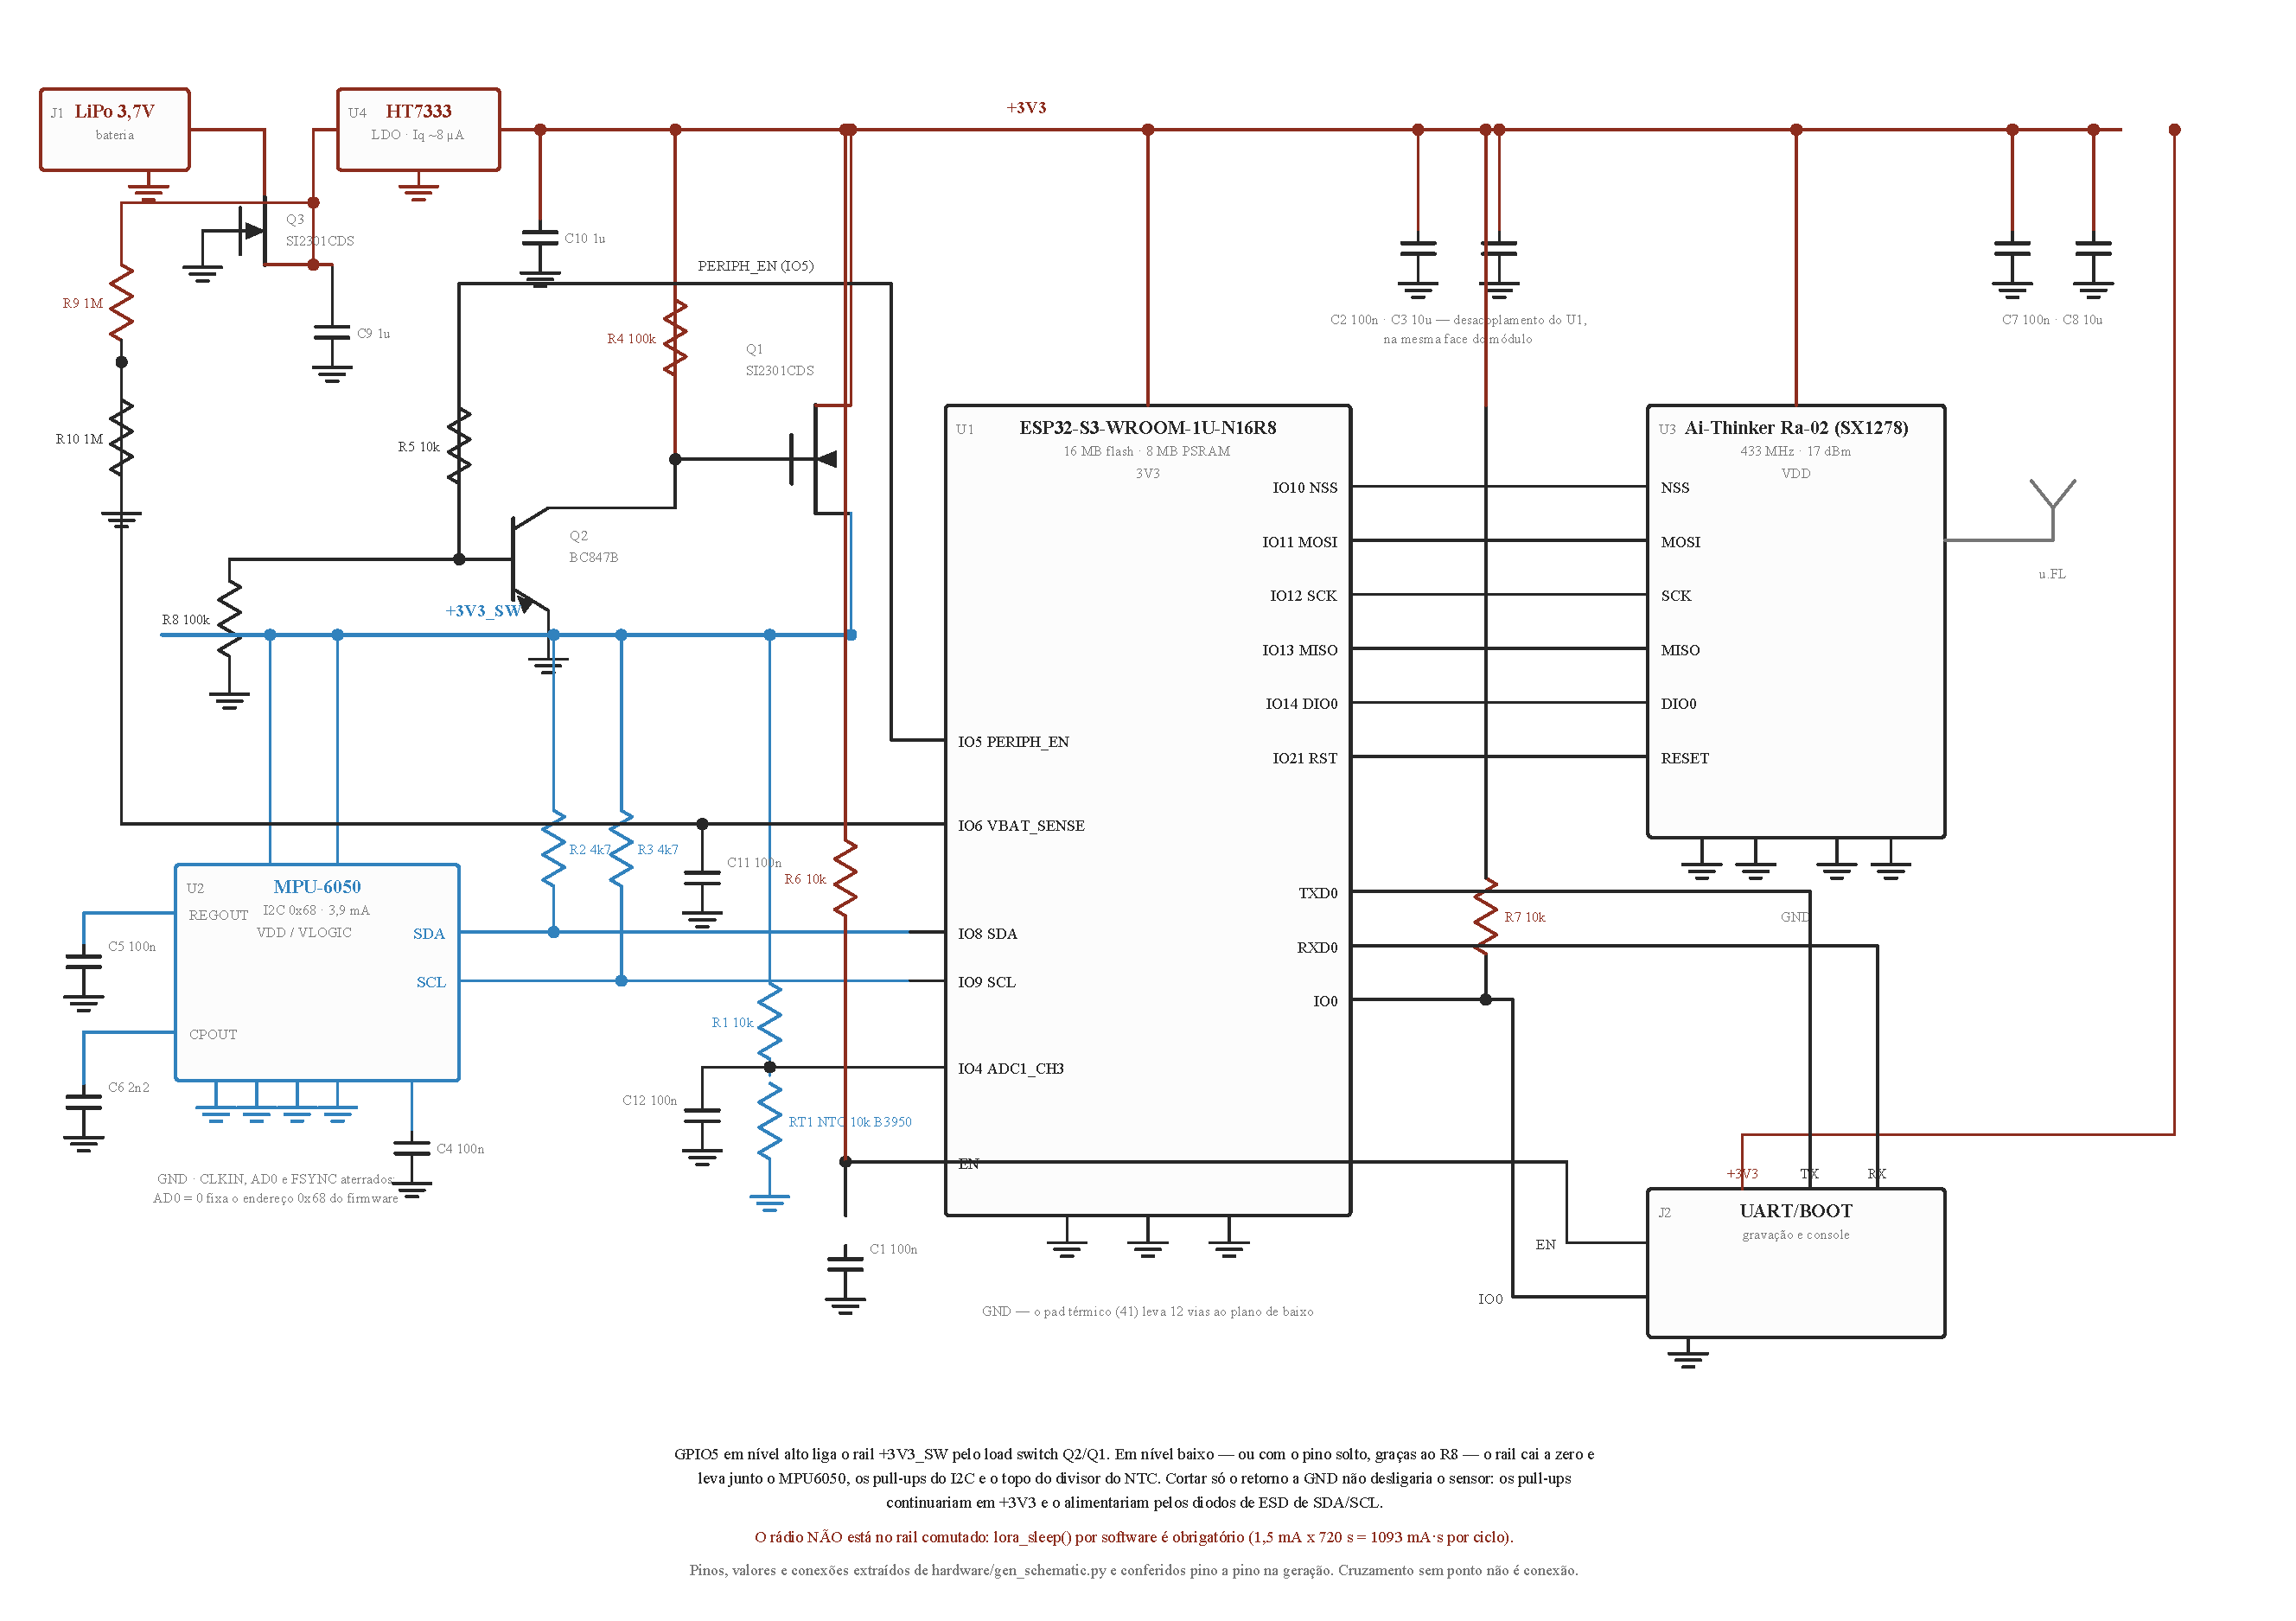
\includegraphics[width=0.88\textwidth]{../../experiments/figures/output/fig8_circuito.pdf}
\caption{Esquemático. A figura é gerada a partir da mesma netlist que produz o
\texttt{.kicad\_sch}, e a geração falha se algum par (referência, pino) da netlist
não estiver desenhado. Confere 106 pinos.}
\end{figure}

\section{Placa gerada}

\begin{figure}[H]\centering
\begin{minipage}{0.24\textwidth}\centering
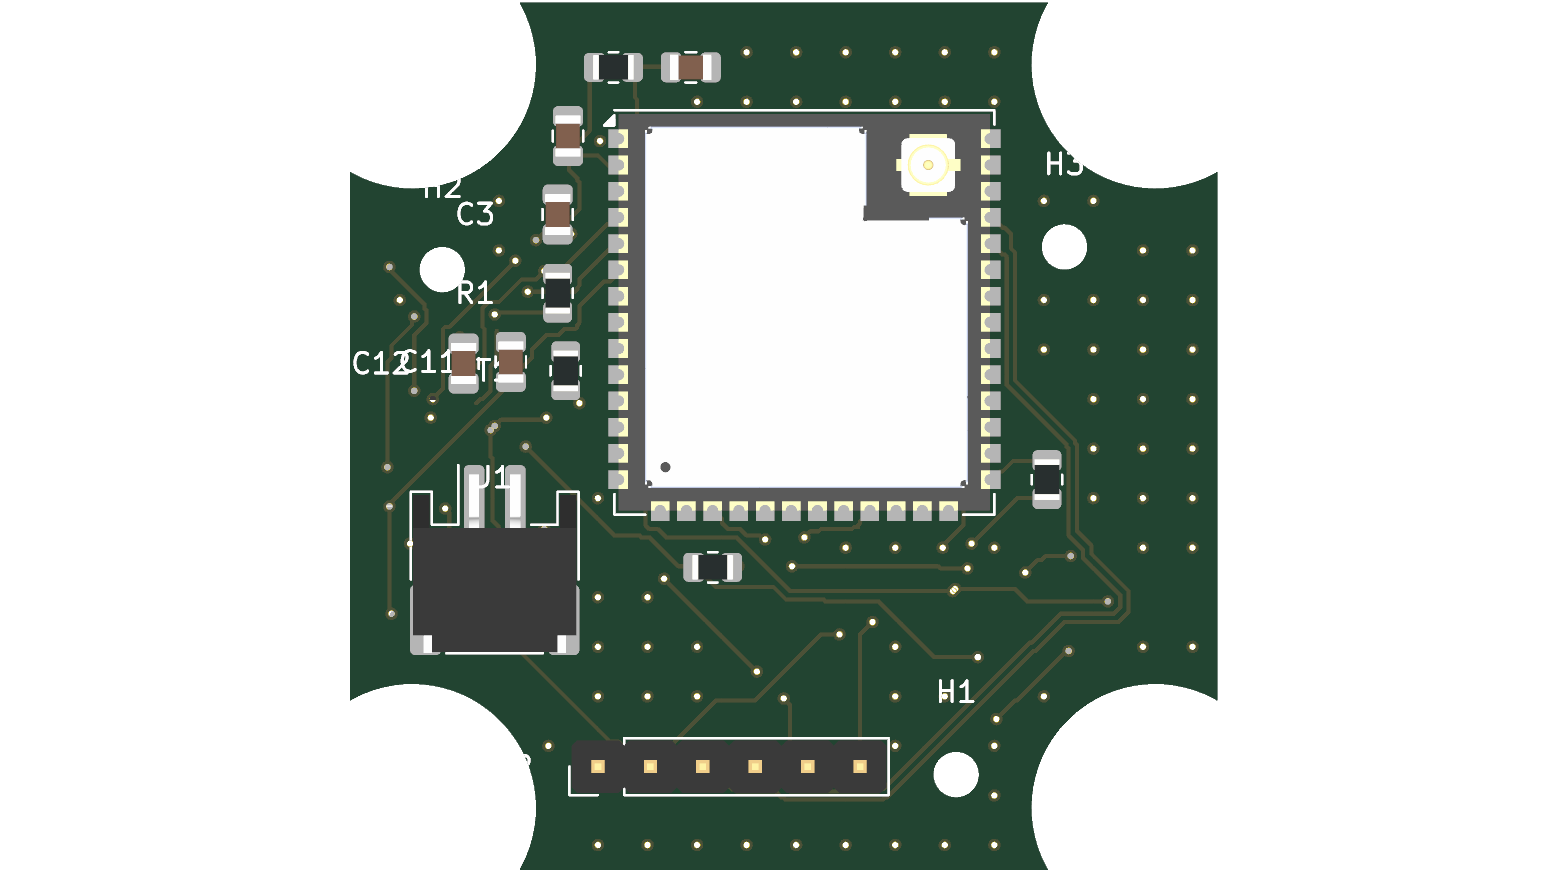
\includegraphics[width=\linewidth]{../../hardware/pcb/v1/render_top.png}\\[1pt]
{\footnotesize v1, face superior}
\end{minipage}\hfill
\begin{minipage}{0.24\textwidth}\centering
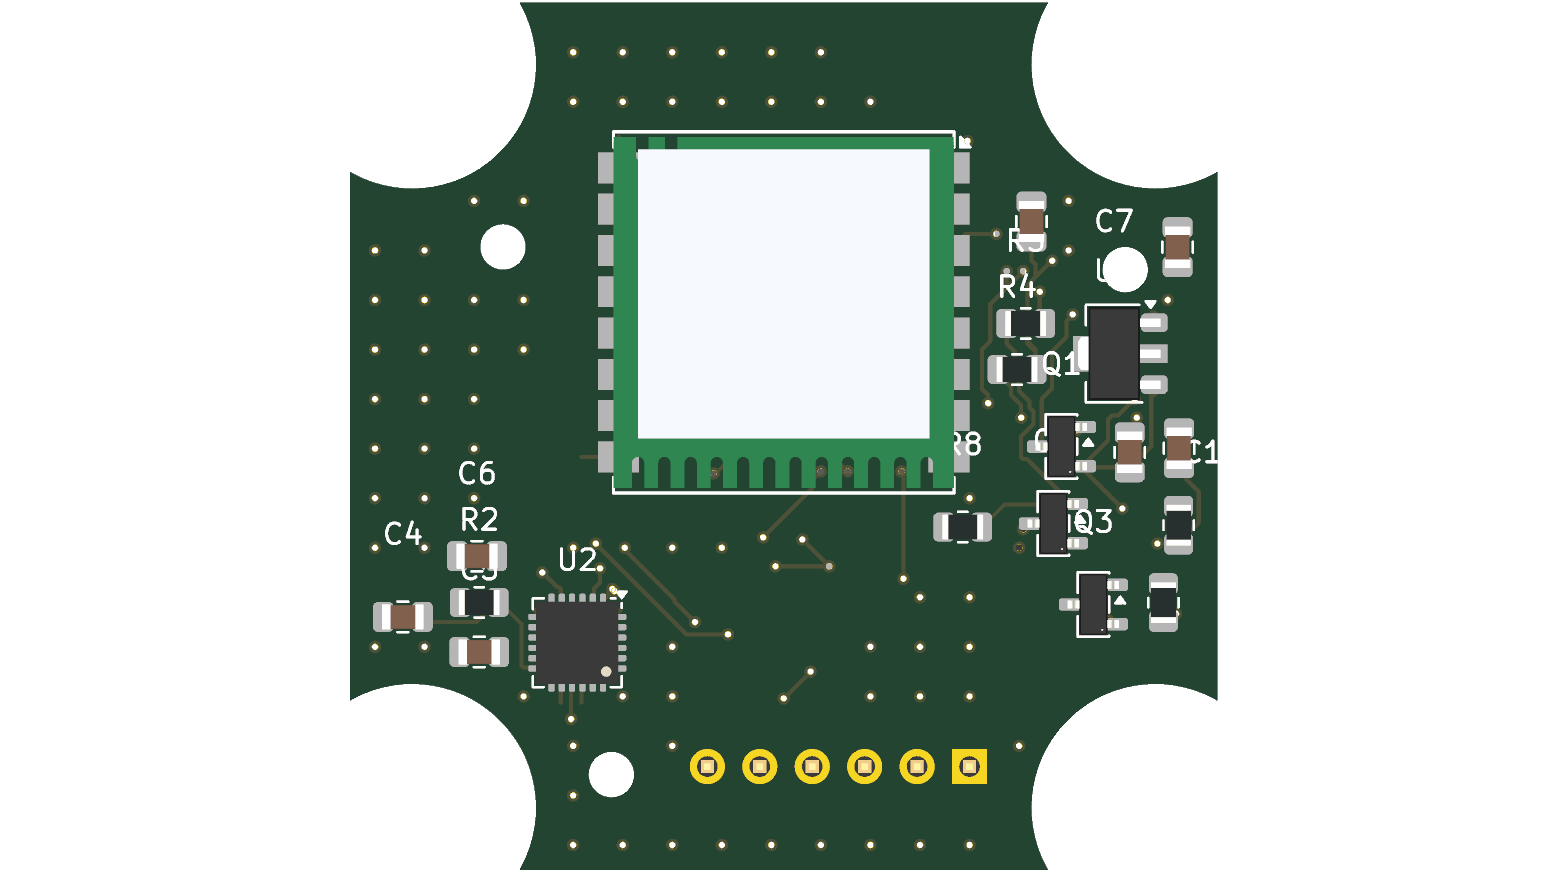
\includegraphics[width=\linewidth]{../../hardware/pcb/v1/render_bottom.png}\\[1pt]
{\footnotesize v1, face inferior}
\end{minipage}\hfill
\begin{minipage}{0.24\textwidth}\centering
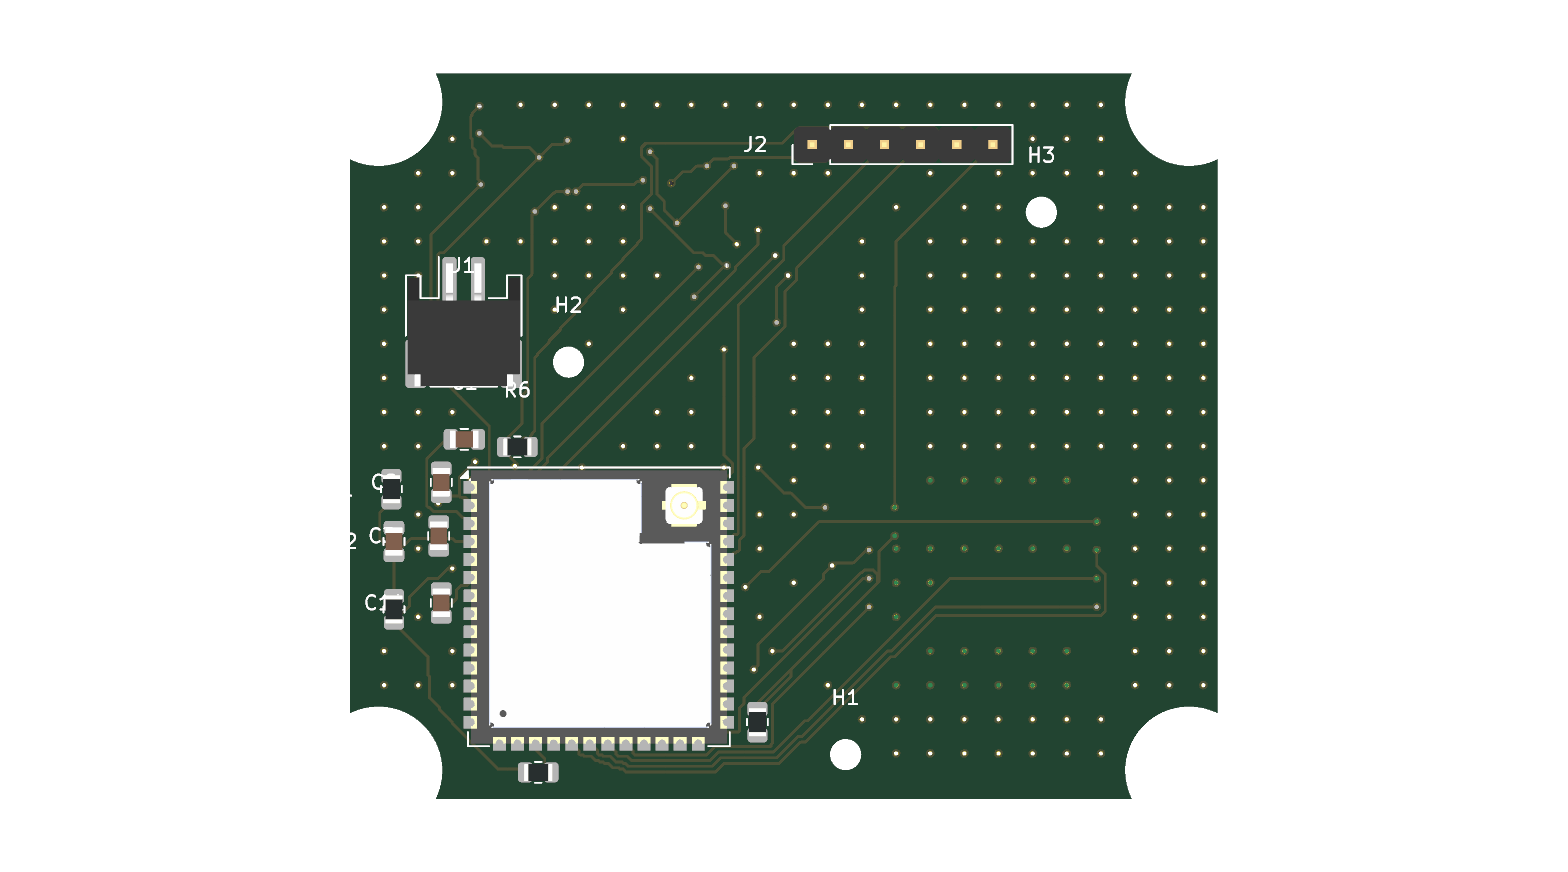
\includegraphics[width=\linewidth]{../../hardware/pcb/v2/render_top.png}\\[1pt]
{\footnotesize v2, face superior}
\end{minipage}\hfill
\begin{minipage}{0.24\textwidth}\centering
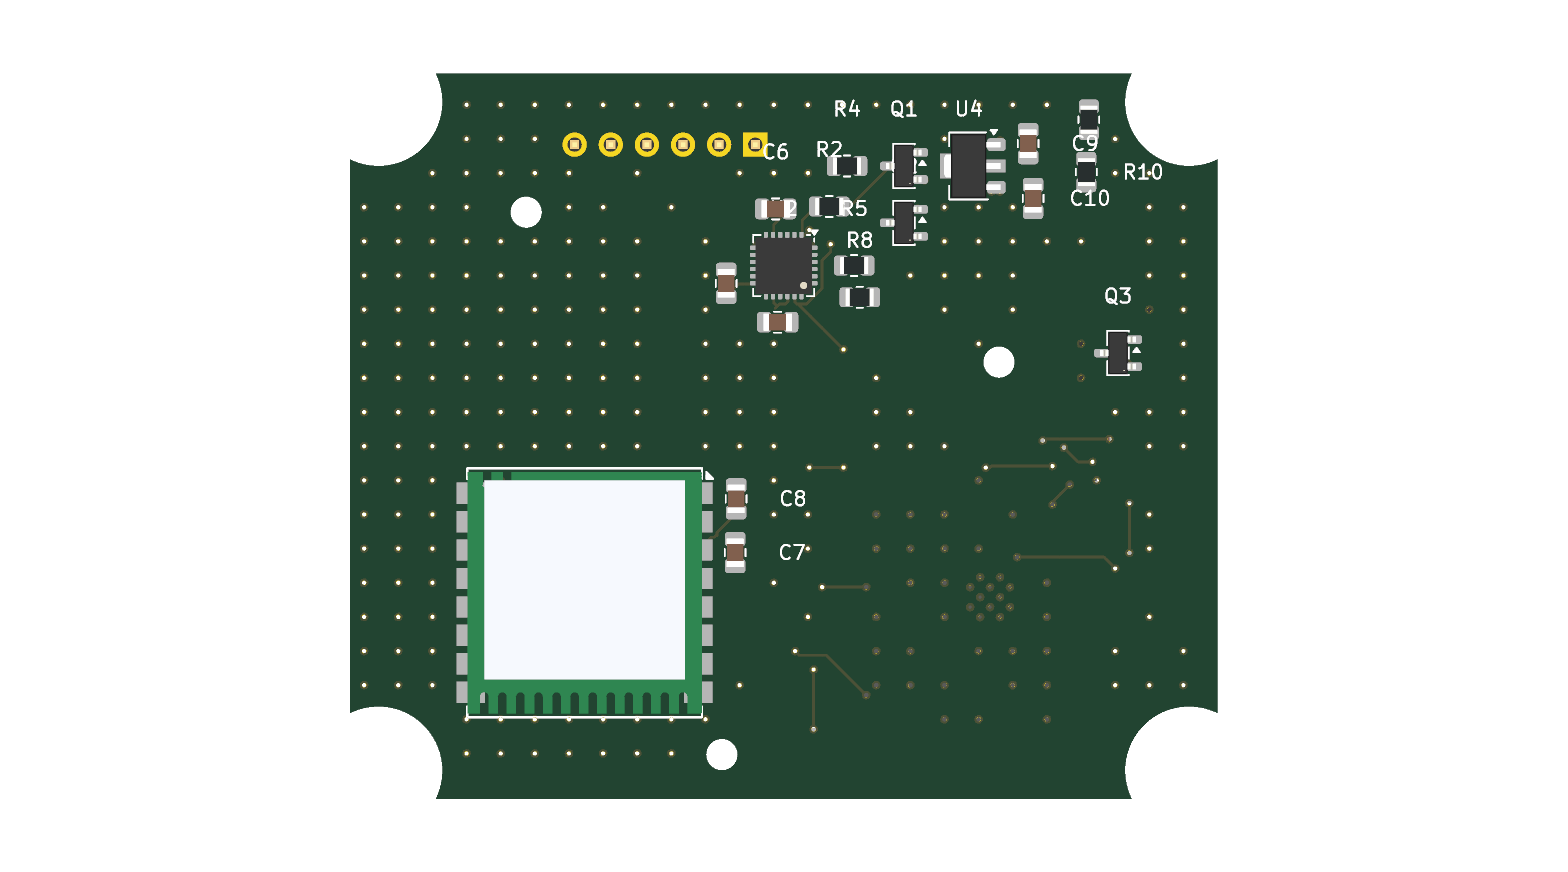
\includegraphics[width=\linewidth]{../../hardware/pcb/v2/render_bottom.png}\\[1pt]
{\footnotesize v2, face inferior}
\end{minipage}
\caption{Placas geradas. Contorno retangular com quatro recortes de canto para
os bosses do invólucro. Duas camadas, plano de terra em ambas.}
\end{figure}

Regras de fabricação, iguais nas duas versões: traço \SI{0.20}{\milli\meter},
folga \SI{0.15}{\milli\meter}, via Ø\SI{0.60}{\milli\meter} com furo
\SI{0.30}{\milli\meter}. Mínimos declarados: furo \SI{0.20}{\milli\meter},
folga \SI{0.15}{\milli\meter}, traço \SI{0.15}{\milli\meter}.

\section{Defeitos de geração da placa}

\subsection{Corrigidos}

\begin{table}[H]\footnotesize
\begin{tabularx}{\textwidth}{@{}p{0.7cm} Y{1.184} Y{0.868} Y{0.947}@{}}
\toprule
\textbf{\#} & \textbf{Defeito} & \textbf{Medição} & \textbf{Correção} \\
\midrule
6  & Ângulo de pad gravado como relativo; é absoluto (biblioteca mais rotação do footprint) & 42 curtos no DRC & conferido contra as placas de exemplo do KiCad \\
7  & Sinal da rotação invertido: pad local $(0;\,7{,}62)$ a \SI{90}{\degree} mapeado para $-x$ & pad 4 do J2 reportado em $+7{,}62$ pelo DRC & sinal corrigido \\
8  & Rotação própria do pad ignorada & QFN-24 descrito com pads de \SI{0.85}{\milli\meter} em passo de \SI{0.5}{\milli\meter}, sobrepostos entre si & largura e altura trocadas quando o pad tem \SI{90}{\degree} \\
9  & Pad \texttt{custom} medido pelo campo \texttt{size} (âncora) & aba do SOT-89 mede \SI{4.6}{\milli\meter}; \texttt{size} declara \SI{1.475}{\milli\meter} & leitura das \texttt{primitives} \\
10 & Colisão mecânica e colisão de cobre tratadas como invariante único & furo M2 sobre o pad do R6 não detectado & invariantes separados; pad passante conta nas duas faces \\
11 & Contorno circular de \SI{74}{\milli\meter} num vão de \SI{43}{\milli\meter}; o verificador comparava escalares & contorno contra vão do desenho & contorno retangular; módulos distribuídos um por face \\
12 & Nenhuma pista roteada & 70 pads desconectados no DRC & roteador de labirinto de duas camadas \\
13 & Corredor de cabo do conector de bateria não modelado & furo M2 a \SI{2.6}{\milli\meter} da boca do conector & corredor incluído como restrição de \emph{placement} \\
\bottomrule
\end{tabularx}
\end{table}

\subsection{Abertos}

\begin{table}[H]\footnotesize
\begin{tabularx}{\textwidth}{@{}p{0.7cm} Y{1.333} Y{0.762} Y{0.762} Y{1.143}@{}}
\toprule
\textbf{\#} & \textbf{Defeito} & \textbf{v1} & \textbf{v2} & \textbf{Decorrência} \\
\midrule
14 & A placa não parafusa nos bosses do invólucro & furo M3 em $(18;\,18)$ exigiria material até \SI{28.2}{\milli\meter} na diagonal; o canto R7 termina em \SI{27.5}{\milli\meter} & recortes $r=\SI{4.5}{\milli\meter}$ coincidem com os eixos dos bosses & a fixação é o assento pelo aro mais três furos M2 próprios \\
15 & Corredor do cabo & \SI{4.0}{\milli\meter} & \SI{6.0}{\milli\meter} & com \SI{6.0}{\milli\meter} a v1 perde a saída de terra de RT1.2 e R8.2 (3 itens soltos no DRC) \\
16 & Altura do conjunto definida pelos conectores & J2 \SI{11.54}{\milli\meter}, J1 \SI{5.60}{\milli\meter}, módulos \SI{3.20}{\milli\meter} & idem & decidir se o header de gravação permanece populado no produto \\
17 & Divisor do NTC satura no frio: \SI{3.22}{\volt} a \SI{-40}{\celsius}, acima da faixa útil do ADC ($\approx$\SI{3.1}{\volt} a \SI{12}{\decibel}) & idem & idem & abaixo de $\approx$\SI{-35}{\celsius} os limiares de curto e aberto não disparam (razão 0,94 contra 0,99) \\
\bottomrule
\end{tabularx}
\end{table}

\begin{table}[H]\footnotesize
\begin{tabularx}{\textwidth}{@{}p{0.7cm} Y{1.333} Y{0.762} Y{0.762} Y{1.143}@{}}
\toprule
\textbf{\#} & \textbf{Defeito} & \textbf{v1} & \textbf{v2} & \textbf{Decorrência} \\
\midrule
18 & Numeração de pino do HT7333 em SOT-89-3 varia por fabricante & \textsf{não verificado} & \textsf{não verificado} & conferir contra a folha de dados antes de fabricar \\
19 & Furo USB-C Ø\SI{13.0}{\milli\meter} no invólucro sem conector correspondente & netlist: J2 é header UART de 6 vias & idem & --- \\
20 & Rabicho u.FL--SMA ausente da BOM & \arq{kaelix-bom.csv} & idem & a ligação do IPEX do Ra-02 ao painel não está especificada \\
21 & Nenhum código lê a tensão da bateria & \texttt{src/} & idem & o caminho de hardware existe; os limiares de REQ-SEG-29 não estão implementados \\
\bottomrule
\end{tabularx}
\end{table}

\section{Versões}

\begin{table}[H]\footnotesize
\begin{tabularx}{\textwidth}{@{}Y{1.1} Y{1.0} Y{1.0} | Y{0.9} Y{1.0}@{}}
\toprule
 & \textbf{Placa v1} & \textbf{Placa v2} & \textbf{Invólucro v1} & \textbf{Invólucro v2} \\
\midrule
Contorno / corpo & $42\times42$, 4 recortes $r=6{,}0$ & $61\times51$, 4 recortes $r=4{,}5$ & $50\times50\times62$ & $69\times59\times38$ \\
Vão interno & --- & --- & $43\times43\times54$ & $62\times52\times30$ \\
Área útil de cobre & \SI{1477}{\milli\meter\squared} & \SI{2962}{\milli\meter\squared} & --- & --- \\
Segmentos (F.Cu / B.Cu) & 478 (327 / 151) & 500 (419 / 81) & --- & --- \\
Vias de sinal / costura & 68 / 92 & 67 / 261 & --- & --- \\
Triedro M2 & \SI{97}{\degree}, 89 ângulos legais & \SI{120}{\degree}, 171 ângulos legais & --- & --- \\
Envelope montado & $42{,}00\times42{,}00\times13{,}42$ & $61{,}00\times51{,}00\times13{,}42$ & --- & --- \\
Folga no vão & --- & --- & \SI{0.50}{\milli\meter} por lado & \SI{0.50}{\milli\meter} por lado \\
Célula que entra & --- & --- & nenhuma de catálogo & Adafruit 2011, \SI{2000}{\milli\ampere\hour} \\
Autonomia a \SI{314}{\micro\ampere} & --- & --- & 66 dias & 265 dias \\
REQ-PWR-06 (243 dias) & --- & --- & não atendido & atendido \\
ERC / DRC & 0 / 0 regra, 0 solto & 0 / 0 regra, 0 solto & --- & --- \\
\bottomrule
\end{tabularx}
\end{table}

Na v1, a interferência da célula Adafruit 1578 (\SI{500}{\milli\ampere\hour}) com os postes Ø\SI{11}{\milli\meter} mede \SI{86.1}{\milli\meter\cubed}. O maior retângulo livre na cavidade v1 é $25\times\SI{40}{\milli\meter}$. Na v2 a interferência da célula de \SI{2000}{\milli\ampere\hour} mede \SI{0.0}{\milli\meter\cubed}.

\subsection{Ausência de assento para a placa}

Seccionando o corpo no plano em que a montagem posiciona a placa (\texttt{FUNDO} $+\ \SI{5.0}{\milli\meter}$), a seção contém a parede externa e os quatro bosses. Não há ressalto, nervura ou batente. A interferência de \SI{0.0}{\milli\meter\cubed} entre placa e corpo indica ausência de contato, não adequação. As condições de contorno das Seções~\ref{sec:modal} e~\ref{sec:vibra} são hipóteses sobre essa indefinição, e a dispersão entre elas quantifica seu efeito.

\section{Rede de alimentação (PDN)}

Impedância vista do pino de alimentação de cada carga, com o comprimento de laço extraído do caminho roteado no \texttt{.kicad\_pcb}. Impedância-alvo $Z_\text{alvo} = \Delta V/\Delta I = \SI{66}{\milli\volt}/\SI{90}{\milli\ampere} = \SI{733}{\milli\ohm}$, com $\Delta I$ igual ao degrau do amplificador de potência do SX1278 e $\Delta V$ correspondente a \SI{2}{\percent} de \SI{3.3}{\volt}. Em duas camadas com plano de retorno a \SI{1.5}{\milli\meter}, a via passante vale \SI{1.30}{\nano\henry} e a pista de \SI{0.2}{\milli\meter}, \SI{781}{\pico\henry\per\milli\meter}.

\begin{table}[H]\footnotesize
\begin{tabularx}{\textwidth}{@{}p{1.0cm} p{0.9cm} p{1.1cm} *{4}{>{\centering\arraybackslash}X} @{}}
\toprule
\textbf{Cap.} & \textbf{Valor} & \textbf{Serve} & \textbf{Distância reta (mm)} & \textbf{Pista roteada (mm)} & \textbf{Vias} & \textbf{$L$ de laço (nH)} \\
\midrule
\multicolumn{7}{@{}l}{\itshape v1} \\
C2  & \SI{100}{\nano\farad} & U1.2  & 2,74  & 2,81  & 0 & 2,19 \\
C3  & \SI{10}{\micro\farad} & U1.2  & 4,63  & 7,03  & 0 & 5,49 \\
C7  & \SI{100}{\nano\farad} & U3.3  & 4,03  & 4,46  & 2 & 6,08 \\
C8  & \SI{10}{\micro\farad} & U3.3  & 11,11 & \textbf{36,06} & \textbf{6} & \textbf{35,95} \\
C10 & \SI{1}{\micro\farad}  & U4.3  & 4,39  & 4,51  & 0 & 3,52 \\
C4  & \SI{100}{\nano\farad} & U2.13 & 6,09  & 8,31  & 0 & 6,49 \\
\addlinespace
\multicolumn{7}{@{}l}{\itshape v2} \\
C2  & \SI{100}{\nano\farad} & U1.2  & 2,42 & 2,31 & 0 & 1,80 \\
C3  & \SI{10}{\micro\farad} & U1.2  & 3,98 & 6,39 & 2 & \textbf{7,59} \\
C7  & \SI{100}{\nano\farad} & U3.3  & 2,82 & 3,06 & 2 & 4,98 \\
C8  & \SI{10}{\micro\farad} & U3.3  & 3,75 & 3,89 & 0 & 3,04 \\
C10 & \SI{1}{\micro\farad}  & U4.3  & 3,11 & 3,30 & 2 & 5,18 \\
C4  & \SI{100}{\nano\farad} & U2.13 & 2,30 & 2,57 & 0 & 2,01 \\
\bottomrule
\end{tabularx}
\end{table}

\begin{table}[H]\footnotesize
\begin{tabularx}{\textwidth}{@{}Y{0.789} Y{1.105} Y{1.105}@{}}
\toprule
\textbf{Carga} & \textbf{v1} & \textbf{v2} \\
\midrule
ESP32-S3 (U1.2, +3V3) & pico \SI{622}{\milli\ohm} em \SI{4.2}{\mega\hertz}; abaixo do alvo em toda a faixa & pico \SI{925}{\milli\ohm} em \SI{6.2}{\mega\hertz}; excede o alvo acima de \SI{6.0}{\mega\hertz} \\
Ra-02 (U3.3, +3V3) & abaixo do alvo em toda a faixa & abaixo do alvo em toda a faixa \\
MPU6050 (U2.13, +3V3\_SW) & abaixo do alvo em toda a faixa & excede o alvo acima de \SI{1.1}{\mega\hertz} \\
\bottomrule
\end{tabularx}
\end{table}

Resultados: (i) a distância em linha reta subestima a indutância de laço em até 3,25$\times$ (C8 na v1); (ii) a métrica anterior de desacoplamento incluía C1, C5, C6 e C9, que não desacoplam rail de alimentação --- C1 é a rede RC do EN, C5 e C6 pertencem ao regulador interno e à bomba de carga do MPU6050, e C9 é o capacitor de entrada do regulador; (iii) a redução da distância em linha reta na v2 não corresponde a redução de impedância: o roteador inseriu duas vias no caminho do capacitor de \emph{bulk} do ESP32-S3, e o laço passou de 5,49 para \SI{7.59}{\nano\henry}.

\begin{figure}[H]\centering
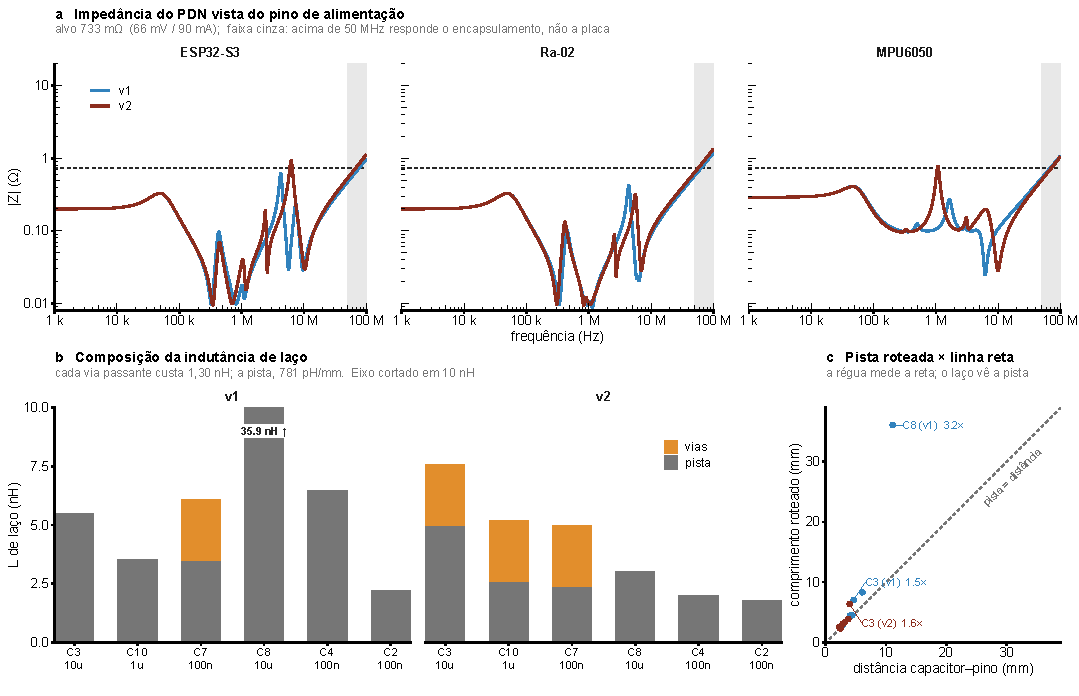
\includegraphics[width=0.96\textwidth]{../../experiments/figures/output/fig9_pdn.pdf}
\caption{Impedância do PDN vista do pino de alimentação de cada carga; composição da indutância de laço; comprimento roteado contra distância em linha reta.}
\end{figure}

\section{Análise modal}
\label{sec:modal}

gmsh 4.15 para malha, CalculiX 2.23 para solução, elementos C3D10. Contorno e furos da placa lidos do \texttt{.kicad\_pcb} gerado.

\begin{table}[H]\footnotesize
\begin{tabularx}{\textwidth}{@{}Y{1.273} Y{0.727} Y{0.727} Y{1.273}@{}}
\toprule
\textbf{Modelo e apoio} & \textbf{v1} & \textbf{v2} & \textbf{Observação} \\
\midrule
Placa, 3 furos M2 engastados, chapa nua & \SI{2951}{\hertz} & \SI{1702}{\hertz} & FR-4 isotrópico, $E=\SI{24}{\giga\pascal}$, $\nu=0{,}136$ \\
Placa, 3 furos M2 engastados, povoada & \SI{2001}{\hertz} & \SI{1352}{\hertz} & massa dos componentes ($+\SI{5.1}{\gram}$) somada como densidade equivalente \\
Placa, aro com apoio simples, povoada & \SI{3986}{\hertz} & \SI{2398}{\hertz} & limite superior \\
Caminho de montagem, carga no piso da cavidade & \SI{1181}{\hertz} & \SI{1670}{\hertz} & ASA maciço, $E=\SI{2.0}{\giga\pascal}$; engaste nos quatro bolsos de ímã \\
Caminho de montagem, carga na borda de cima & \SI{936}{\hertz} & \SI{679}{\hertz} & hipótese de \arq{analise-involucro.ipynb} \\
\bottomrule
\end{tabularx}
\end{table}

O modo relatado para o caminho de montagem é o de maior massa modal efetiva lateral (41--\SI{69}{\gram} de $\approx$\SI{110}{\gram}), não o primeiro autovalor: em vários casos o primeiro modo é local de parede e não desloca o sensor.

\begin{table}[H]\footnotesize
\begin{tabularx}{\textwidth}{@{}Y{1.2} Y{0.9} Y{0.9} Y{1.0}@{}}
\toprule
\textbf{Tamanho de elemento} & \textbf{v1, carga no topo} & \textbf{v2, carga no topo} & \textbf{Nós (v2)} \\
\midrule
\SI{3.5}{\milli\meter} & \SI{936}{\hertz} & \SI{679}{\hertz} & 27\,346 \\
\SI{2.5}{\milli\meter} & \SI{922}{\hertz} & \SI{641}{\hertz} & 55\,181 \\
\SI{1.8}{\milli\meter} & \SI{927}{\hertz} & \SI{657}{\hertz} & 123\,817 \\
\bottomrule
\end{tabularx}
\caption*{\footnotesize Dispersão de \SI{1.5}{\percent} (v1) e \SI{6}{\percent} (v2). As conclusões não dependem do refino.}
\end{table}

As formas modais indicam mecanismos distintos entre as versões. Na v1 o caminho apresenta flexão de viga engastada, com deslocamento crescente com a altura e máximo na borda superior. Na v2 a base permanece praticamente imóvel e o deslocamento concentra-se na borda superior, em dois cantos opostos: a redução de altura de 62 para \SI{38}{\milli\meter} enrijeceu a coluna e o alargamento dos painéis de $50\times50$ para $69\times59$ transferiu a flexibilidade para a borda.

\begin{figure}[H]\centering
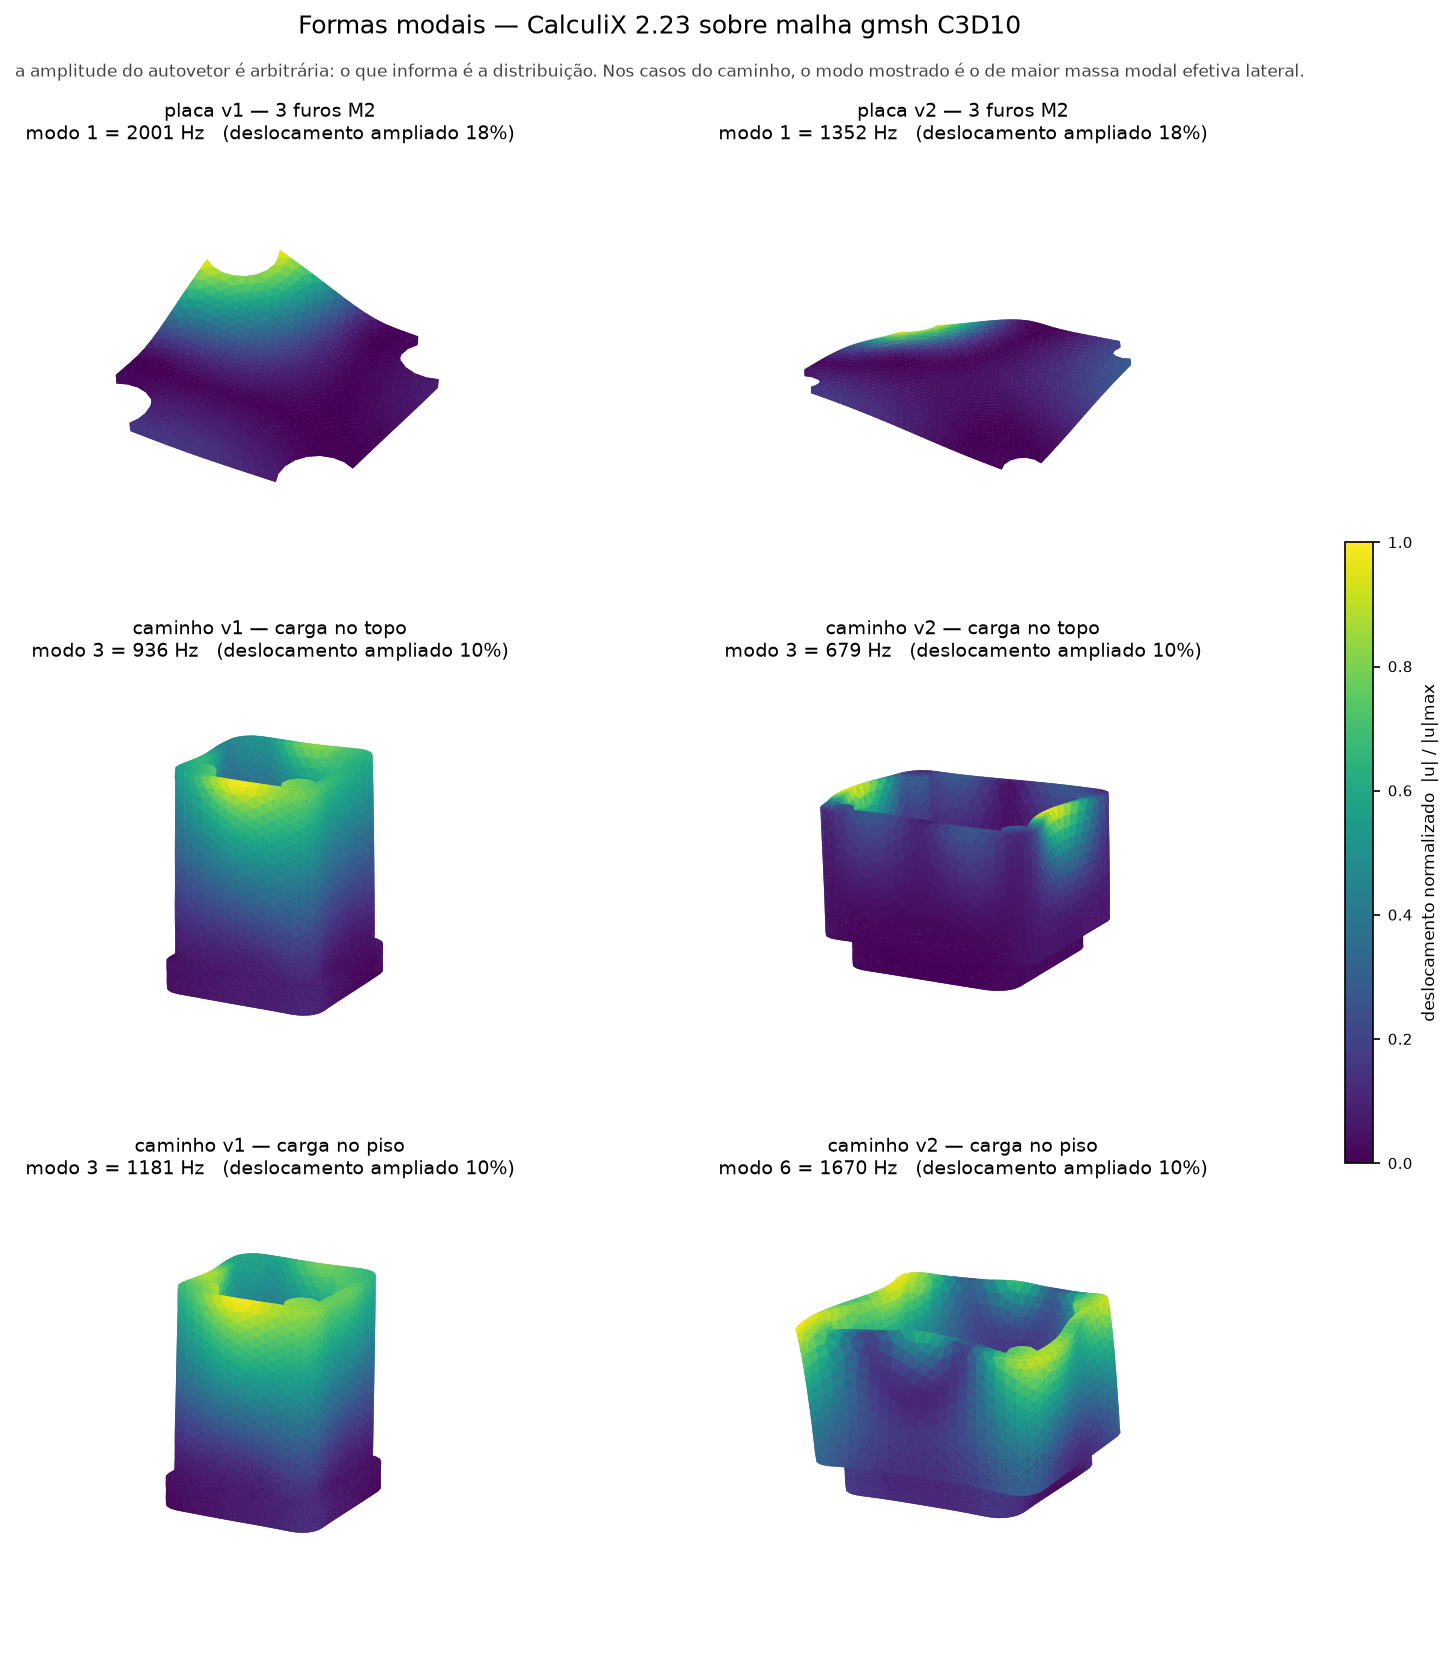
\includegraphics[height=0.80\textheight]{../../hardware/fem/figuras/modos.png}
\caption{Formas modais da placa e do caminho de montagem. A amplitude do autovetor é arbitrária; a informação está na distribuição.}
\end{figure}

\section{Vibração aleatória e fadiga de junta de solda}
\label{sec:vibra}

Excitação derivada da ISO 10816-3, classe III, limiar C/D $=\SI{11.2}{\milli\meter\per\second}$ RMS, com os limites importados de \arq{kaelix\_ml/labeling.py}. Densidade espectral de velocidade constante na banda de 10 a \SI{1000}{\hertz}. Resposta pela equação de Miles com $Q=\sqrt{f_n}$. Critério de deslocamento admissível de Steinberg,
\[
Z_\text{adm} = \frac{0{,}00022\,B}{c\,h\,\sqrt{L}}\quad\text{[polegadas]},
\]
para $2\times10^{7}$ ciclos, com expoente S-N da solda $b=6{,}4$.

\begin{table}[H]\footnotesize
\begin{tabularx}{\textwidth}{@{}Y{1.2} Y{0.9} Y{0.9}@{}}
\toprule
 & \textbf{v1} & \textbf{v2} \\
\midrule
Primeiro modo da placa & \SI{2001}{\hertz} & \SI{1352}{\hertz} \\
PSD de aceleração nessa frequência\footnotemark[1] & \num{0.208}~$g^{2}$/Hz & \num{0.095}~$g^{2}$/Hz \\
Deslocamento $3\sigma$ máximo & \SI{31.8}{\micro\meter} & \SI{35.1}{\micro\meter} \\
Componente de menor margem & J2 & U1 \\
Margem com base rígida & 7,3$\times$ & 4,2$\times$ \\
Margem sem escalonamento pela forma modal & 2,4$\times$ & 2,7$\times$ \\
\bottomrule
\end{tabularx}
\footnotetext[1]{$g$ denota a aceleração da gravidade padrão, \SI{9.80665}{\meter\per\second\squared}.}
\end{table}

Com base rígida todos os componentes satisfazem o critério. A hipótese de base rígida exige que placa e chassi estejam separados por um fator 2 (regra da oitava de Steinberg). A condição não é satisfeita em três das quatro combinações.

\begin{table}[H]\footnotesize
\begin{tabularx}{\textwidth}{@{}Y{1.500} Y{0.875} Y{0.750} Y{0.750} Y{1.000} Y{1.125} Y{1.000}@{}}
\toprule
\textbf{Combinação} & \textbf{$f$ do chassi} & \textbf{Razão} & \textbf{$T$} & \textbf{Margem corrigida} & \textbf{Vida em zona C/D contínua} & \textbf{Regra da oitava} \\
\midrule
v1, carga no topo & \SI{936}{\hertz}  & 2,14 & 0,28 & 26,0$\times$ & $>$ 100 anos & \ok \\
v1, carga no piso & \SI{1181}{\hertz} & 1,69 & 0,54 & 13,7$\times$ & $>$ 100 anos & \nok \\
v2, carga no topo & \SI{679}{\hertz}  & 1,99 & 0,34 & 12,3$\times$ & $>$ 100 anos & \nok \\
\textbf{v2, carga no piso} & \textbf{\SI{1670}{\hertz}} & \textbf{0,81} & \textbf{2,88} & \textbf{1,4$\times$} & \textbf{43 h} & \nok \\
\bottomrule
\end{tabularx}
\caption*{\footnotesize $T$: transmissibilidade do chassi na frequência da placa, com $\zeta=0{,}03$ para o ASA. A última linha corresponde à configuração implicada pela montagem atual.}
\end{table}

Dois fatores concorrem na v2: o aumento da placa reduziu o primeiro modo de 2001 para \SI{1352}{\hertz}, e o U1 passou de amplitude modal local 0,21 para 0,65. A correção por transmissibilidade é aproximação: Miles com um grau de liberdade pressupõe base rígida, e a regra da oitava não é satisfeita. Uma análise acoplada placa--invólucro exige definir previamente a fixação da placa.

Sensibilidade da margem do pior caso, sem a correção do chassi (v1 / v2): $Q=10$, 15,5$\times$ / 8,0$\times$; $Q=20$, 11,0$\times$ / 5,6$\times$; $Q=\sqrt{f_n}$, 7,3$\times$ / 4,2$\times$ na zona C/D. A ordem entre as versões não se altera.

\begin{figure}[H]\centering
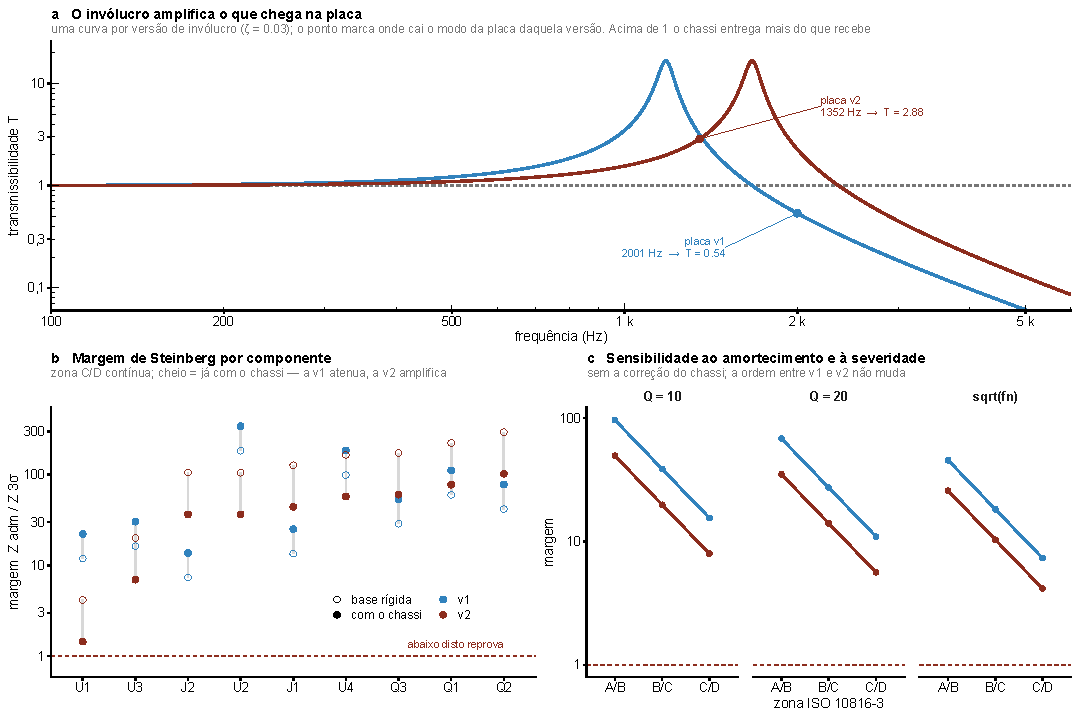
\includegraphics[width=0.96\textwidth]{../../experiments/figures/output/fig10_vibracao.pdf}
\caption{Transmissibilidade do caminho de montagem, margem de Steinberg por componente e sensibilidade ao amortecimento e à severidade.}
\end{figure}

\section{Condução térmica do motor à placa}

Invólucro fechado (base, corpo e tampa) em ASA, $k=\SI{0.17}{\watt\per\meter\per\kelvin}$. Entrada pelos quatro bolsos de ímã presos a \SI{90}{\celsius}. Convecção natural e radiação linearizada para \SI{30}{\celsius} nas faces externas. Cavidade adiabática.

\begin{table}[H]\footnotesize
\begin{tabularx}{\textwidth}{@{}p{1.0cm} *{5}{>{\centering\arraybackslash}X}@{}}
\toprule
 & \textbf{Ímã} & \textbf{Base, $z\approx\SI{3}{\milli\meter}$} & \textbf{Meia altura} & \textbf{Tampa} & \textbf{Parede da cavidade} \\
\midrule
v1 & \SI{90.0}{\celsius} & \SI{57.0}{\celsius} & \SI{31.4}{\celsius} & \SI{30.0}{\celsius} & \SI{34.3}{\celsius} \\
v2 & \SI{90.0}{\celsius} & \SI{58.2}{\celsius} & \SI{32.6}{\celsius} & \SI{30.1}{\celsius} & \SI{35.1}{\celsius} \\
\bottomrule
\end{tabularx}
\end{table}

A resistência de entrada mede $\approx\SI{118}{\kelvin\per\watt}$ (\SI{12.3}{\milli\meter} de ASA sobre \SI{615}{\milli\meter\squared}) contra $\approx\SI{5}{\kelvin\per\watt}$ de troca com o ar. Dos \SI{60}{\kelvin} de salto, \SI{33}{\kelvin} ocorrem nos primeiros \SI{4}{\milli\meter} da base. O fluxo mede \SI{640}{\milli\watt}.

A cavidade não é isotérmica. A placa assenta \SI{5.0}{\milli\meter} acima do piso, com fator de forma 0,80 (v1) e 0,84 (v2) para ele.

\begin{table}[H]\footnotesize
\begin{tabularx}{\textwidth}{@{}p{1.0cm} *{5}{>{\centering\arraybackslash}X}@{}}
\toprule
 & \textbf{Piso da cavidade} & \textbf{Paredes} & \textbf{Tampa} & \textbf{Média} & \textbf{Placa, equilíbrio radiativo} \\
\midrule
v1 & \SI{49.1}{\celsius} & \SI{31.9}{\celsius} & \SI{30.0}{\celsius} & \SI{34.3}{\celsius} & \SI{38.6}{\celsius} \\
v2 & \SI{48.2}{\celsius} & \SI{31.7}{\celsius} & \SI{30.1}{\celsius} & \SI{35.1}{\celsius} & \SI{38.3}{\celsius} \\
\bottomrule
\end{tabularx}
\end{table}

Margem para o limite de carga da célula de lítio-polímero (\SI{45}{\celsius}): \SI{6.5}{\kelvin} com a carcaça a \SI{90}{\celsius}. Transiente após degrau de 30 para \SI{90}{\celsius}: $\tau=\SI{23}{\minute}$ (v1) e \SI{24}{\minute} (v2); \SI{90}{\percent} do salto em 50 e \SI{53}{\minute}; \SI{99}{\percent} em 113 e \SI{120}{\minute}. A massa térmica interna (20 e \SI{50}{\joule\per\kelvin}) contribui com 4 e \SI{7}{\minute} próprios.

\begin{figure}[H]\centering
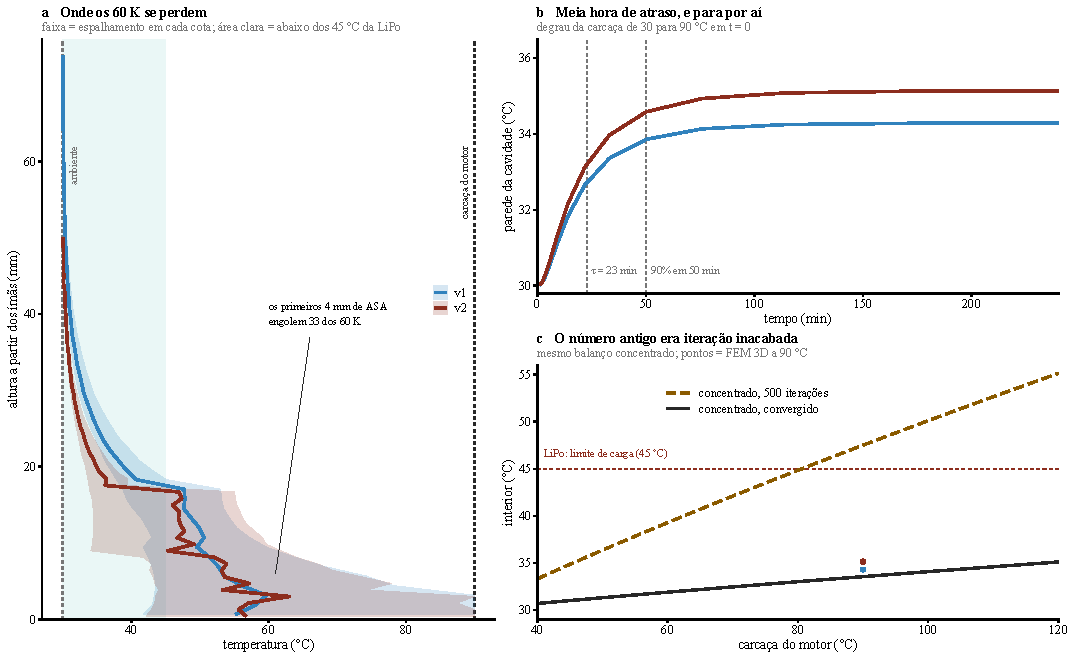
\includegraphics[width=0.94\textwidth]{../../experiments/figures/output/fig11_termica3d.pdf}
\caption{Perfil de temperatura ao longo da altura, transiente da parede da cavidade e comparação com o modelo concentrado.}
\end{figure}

\begin{figure}[H]\centering
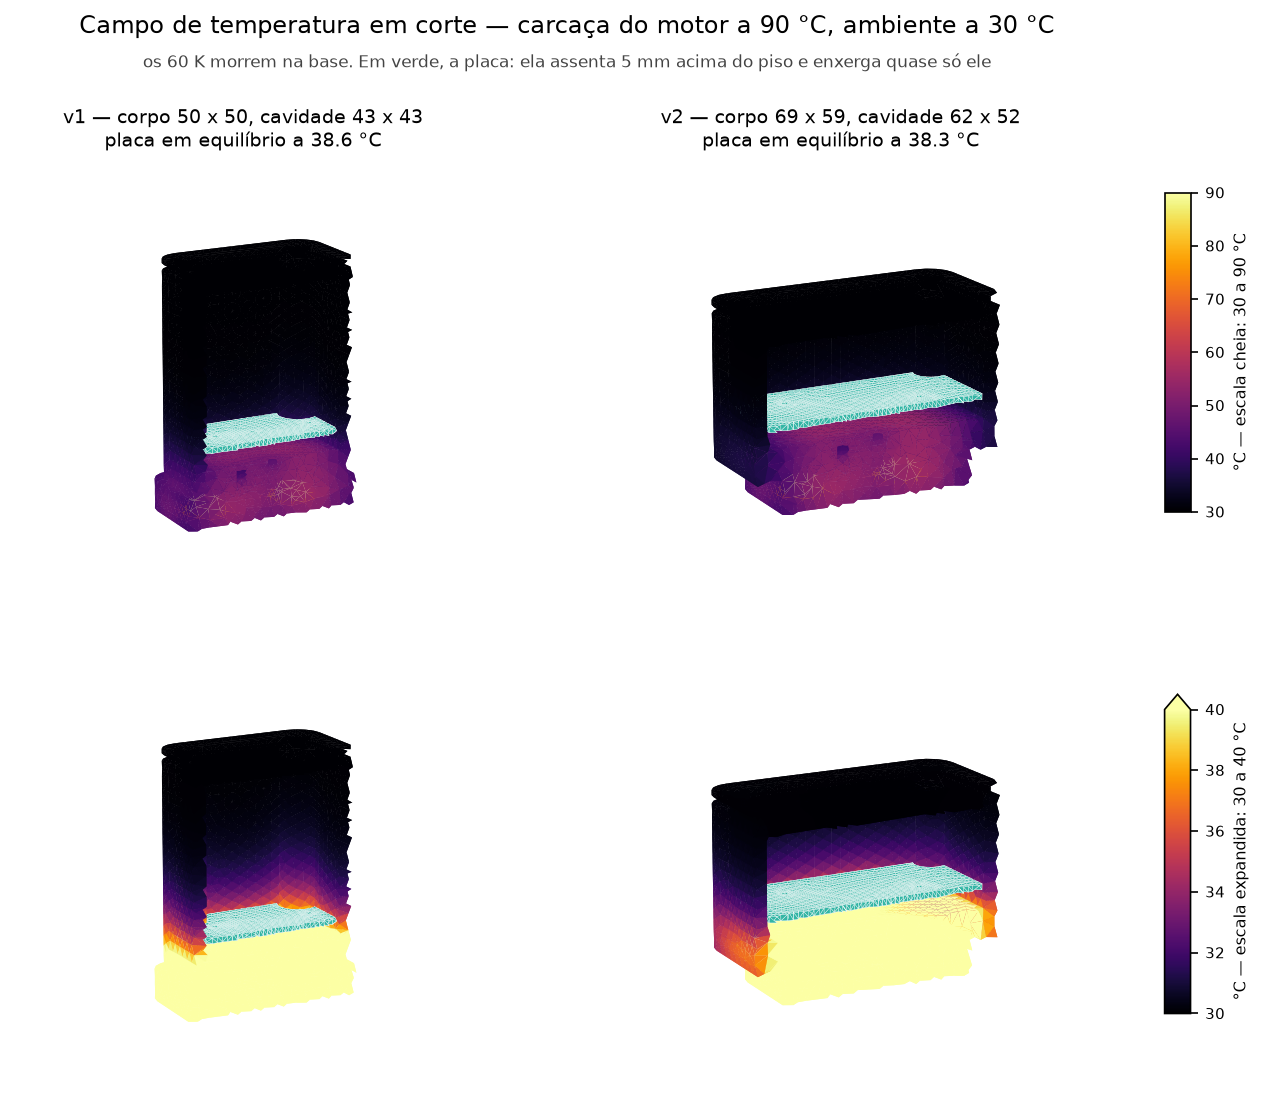
\includegraphics[height=0.60\textheight]{../../hardware/fem/figuras/termica.png}
\caption{Campo de temperatura em corte. A placa (em verde) não integra o modelo de elementos finitos; sua temperatura provém do balanço radiativo separado.}
\end{figure}

\section{Correções a análises anteriores}
\label{sec:correcoes}

\begin{table}[H]\footnotesize
\begin{tabularx}{\textwidth}{@{}Y{0.952} Y{1.238} Y{0.857} Y{0.952}@{}}
\toprule
\textbf{Origem} & \textbf{Causa} & \textbf{Valor anterior} & \textbf{Valor corrigido} \\
\midrule
\arq{analise-termica.ipynb}, função \texttt{temp\_corpo} & iteração de ganho fixo (\num{0.005}) com 500 passos; o resíduo do balanço no passo 500 mede \SI{2831}{\milli\watt}, cerca de cinco vezes o fluxo & \SI{44.8}{\celsius} a \SI{80}{\celsius} de carcaça; \SI{47.5}{\celsius} a \SI{90}{\celsius} & \SI{33.0}{\celsius} e \SI{33.5}{\celsius} \\
\texttt{gen\_pcb.py}, comentário da varredura do corredor & varredura medida antes das correções 6, 8 e 9 & limite atribuído ao triedro de furos e a passivos sem lugar & o \emph{placement} fecha de 2,0 a \SI{9.0}{\milli\meter}; o limite é a continuidade do plano de terra \\
\texttt{gen\_pcb.py}, lista \texttt{\_DESACOPLA} & incluía capacitores que não desacoplam rail de alimentação & 10 capacitores medidos & 6 capacitores \\
Esta análise, temperatura da placa & uso da média da cavidade, que não é isotérmica & \SI{34.3}{\celsius} / \SI{35.1}{\celsius} & \SI{38.6}{\celsius} / \SI{38.3}{\celsius} \\
\bottomrule
\end{tabularx}
\end{table}

O erro de \texttt{temp\_corpo} afeta apenas os ramos de alta resistência. O ramo de alumínio ($R=\SI{0.07}{\kelvin\per\watt}$) converge, e seus \SI{79.0}{\celsius} permanecem válidos; a conclusão de que a base metálica degrada o isolamento térmico não se altera. Alteram-se as margens: a \SI{33}{\celsius} a célula apresenta \SI{12}{\kelvin} de folga sobre o limite de carga, e a curva convergida não cruza \SI{45}{\celsius} na faixa avaliada.

\section{Limitações declaradas}

\begin{table}[H]\footnotesize
\begin{tabularx}{\textwidth}{@{}Y{0.600} Y{1.286} Y{1.114}@{}}
\toprule
\textbf{Análise} & \textbf{Simplificação} & \textbf{Direção do erro} \\
\midrule
Modal & ASA isotrópico e maciço, $E=\SI{2.0}{\giga\pascal}$ & otimista: peça impressa a \SI{35}{\percent} de preenchimento é anisotrópica e menos rígida \\
Modal & junta do spigot tratada como colada & otimista: base e corpo são aparafusados, com \SI{0.2}{\milli\meter} de folga radial \\
Modal & nós de meio-lado lineares & perda de fidelidade em faces curvas; adotado porque a projeção invertia elementos \\
Modal & massa dos componentes distribuída na chapa & subestima a queda quando a massa está no meio do vão \\
Vibração & densidade espectral de velocidade constante extrapolada acima de \SI{1}{\kilo\hertz} & conservador: espectro de máquina decai em velocidade acima de algumas centenas de hertz \\
Vibração & $\zeta=0{,}03$ para o ASA & não medido; herdado de \arq{analise-involucro.ipynb} \\
Vibração & $c=2{,}25$ para módulos e QFN & classe sem terminal, a mais restritiva de Steinberg; com $c=1{,}26$ as margens dobram \\
Térmica & face do bolso de ímã presa a \SI{90}{\celsius} & otimista: ímã real apresenta cola e resistência de contato \\
Térmica & cavidade adiabática na condução & condução pelo ar excede \SI{1000}{\kelvin\per\watt} contra poucos \si{\kelvin\per\watt} da parede \\
Térmica & equilíbrio da placa por média ponderada por fator de forma, $\epsilon\to1$ & ignora a mistura do ar; o valor real situa-se entre 35 e \SI{38.5}{\celsius} \\
PDN & impedância de saída do HT7333 estimada em \SI{0.2}{\ohm} até \SI{50}{\kilo\hertz} & ordem de grandeza; a folha de dados não publica curva de $Z_\text{out}$ \\
PDN & modelo válido até $\approx\SI{50}{\mega\hertz}$ & acima disso responde o encapsulamento, ausente do modelo \\
\bottomrule
\end{tabularx}
\end{table}

\end{document}
